\documentclass[1p]{elsarticle_modified}
%\bibliographystyle{elsarticle-num}

%\usepackage[colorlinks]{hyperref}
%\usepackage{abbrmath_seonhwa} %\Abb, \Ascr, \Acal ,\Abf, \Afrak
\usepackage{amsfonts}
\usepackage{amssymb}
\usepackage{amsmath}
\usepackage{amsthm}
\usepackage{scalefnt}
\usepackage{amsbsy}
\usepackage{kotex}
\usepackage{caption}
\usepackage{subfig}
\usepackage{color}
\usepackage{graphicx}
\usepackage{xcolor} %% white, black, red, green, blue, cyan, magenta, yellow
\usepackage{float}
\usepackage{setspace}
\usepackage{hyperref}

\usepackage{tikz}
\usetikzlibrary{arrows}

\usepackage{multirow}
\usepackage{array} % fixed length table
\usepackage{hhline}

%%%%%%%%%%%%%%%%%%%%%
\makeatletter
\renewcommand*\env@matrix[1][\arraystretch]{%
	\edef\arraystretch{#1}%
	\hskip -\arraycolsep
	\let\@ifnextchar\new@ifnextchar
	\array{*\c@MaxMatrixCols c}}
\makeatother %https://tex.stackexchange.com/questions/14071/how-can-i-increase-the-line-spacing-in-a-matrix
%%%%%%%%%%%%%%%

\usepackage[normalem]{ulem}

\newcommand{\msout}[1]{\ifmmode\text{\sout{\ensuremath{#1}}}\else\sout{#1}\fi}
%SOURCE: \msout is \stkout macro in https://tex.stackexchange.com/questions/20609/strikeout-in-math-mode

\newcommand{\cancel}[1]{
	\ifmmode
	{\color{red}\msout{#1}}
	\else
	{\color{red}\sout{#1}}
	\fi
}

\newcommand{\add}[1]{
	{\color{blue}\uwave{#1}}
}

\newcommand{\replace}[2]{
	\ifmmode
	{\color{red}\msout{#1}}{\color{blue}\uwave{#2}}
	\else
	{\color{red}\sout{#1}}{\color{blue}\uwave{#2}}
	\fi
}

\newcommand{\Sol}{\mathcal{S}} %segment
\newcommand{\D}{D} %diagram
\newcommand{\A}{\mathcal{A}} %arc


%%%%%%%%%%%%%%%%%%%%%%%%%%%%%5 test

\def\sl{\operatorname{\textup{SL}}(2,\Cbb)}
\def\psl{\operatorname{\textup{PSL}}(2,\Cbb)}
\def\quan{\mkern 1mu \triangleright \mkern 1mu}

\theoremstyle{definition}
\newtheorem{thm}{Theorem}[section]
\newtheorem{prop}[thm]{Proposition}
\newtheorem{lem}[thm]{Lemma}
\newtheorem{ques}[thm]{Question}
\newtheorem{cor}[thm]{Corollary}
\newtheorem{defn}[thm]{Definition}
\newtheorem{exam}[thm]{Example}
\newtheorem{rmk}[thm]{Remark}
\newtheorem{alg}[thm]{Algorithm}

\newcommand{\I}{\sqrt{-1}}
\begin{document}

%\begin{frontmatter}
%
%\title{Boundary parabolic representations of knots up to 8 crossings}
%
%%% Group authors per affiliation:
%\author{Yunhi Cho} 
%\address{Department of Mathematics, University of Seoul, Seoul, Korea}
%\ead{yhcho@uos.ac.kr}
%
%
%\author{Seonhwa Kim} %\fnref{s_kim}}
%\address{Center for Geometry and Physics, Institute for Basic Science, Pohang, 37673, Korea}
%\ead{ryeona17@ibs.re.kr}
%
%\author{Hyuk Kim}
%\address{Department of Mathematical Sciences, Seoul National University, Seoul 08826, Korea}
%\ead{hyukkim@snu.ac.kr}
%
%\author{Seokbeom Yoon}
%\address{Department of Mathematical Sciences, Seoul National University, Seoul, 08826,  Korea}
%\ead{sbyoon15@snu.ac.kr}
%
%\begin{abstract}
%We find all boundary parabolic representation of knots up to 8 crossings.
%
%\end{abstract}
%\begin{keyword}
%    \MSC[2010] 57M25 
%\end{keyword}
%
%\end{frontmatter}

%\linenumbers
%\tableofcontents
%
\newcommand\colored[1]{\textcolor{white}{\rule[-0.35ex]{0.8em}{1.4ex}}\kern-0.8em\color{red} #1}%
%\newcommand\colored[1]{\textcolor{white}{ #1}\kern-2.17ex	\textcolor{white}{ #1}\kern-1.81ex	\textcolor{white}{ #1}\kern-2.15ex\color{red}#1	}

{\Large $\underline{12a_{0140}~(K12a_{0140})}$}

\setlength{\tabcolsep}{10pt}
\renewcommand{\arraystretch}{1.6}
\vspace{1cm}\begin{tabular}{m{100pt}>{\centering\arraybackslash}m{274pt}}
\multirow{5}{120pt}{
	\centering
	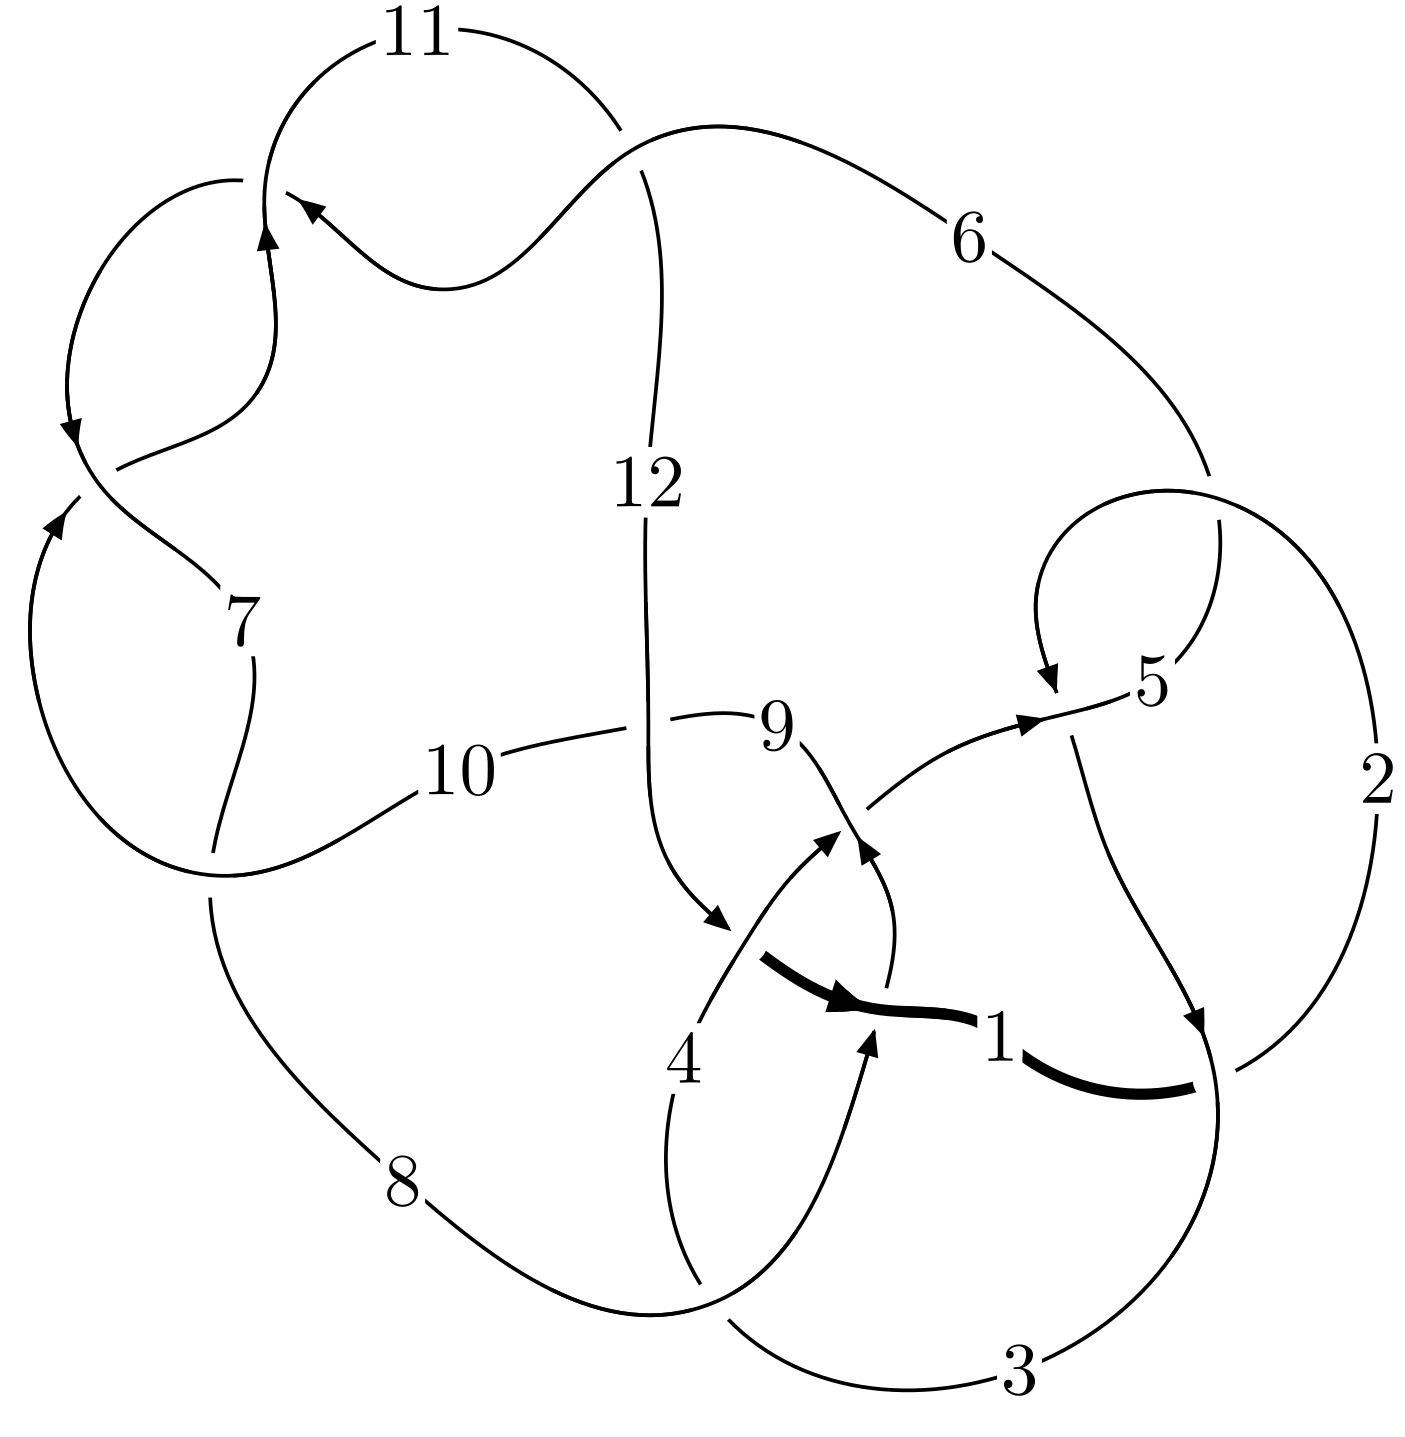
\includegraphics[width=112pt]{../../../GIT/diagram.site/Diagrams/png/941_12a_0140.png}\\
\ \ \ A knot diagram\footnotemark}&
\allowdisplaybreaks
\textbf{Linearized knot diagam} \\
\cline{2-2}
 &
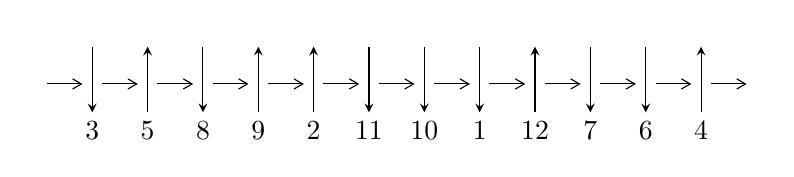
\begin{tikzpicture}[x=20pt, y=17pt]
	% nodes
	\node (C0) at (0, 0) {};
	\node (C1) at (1, 0) {};
	\node (C1U) at (1, +1) {};
	\node (C1D) at (1, -1) {3};

	\node (C2) at (2, 0) {};
	\node (C2U) at (2, +1) {};
	\node (C2D) at (2, -1) {5};

	\node (C3) at (3, 0) {};
	\node (C3U) at (3, +1) {};
	\node (C3D) at (3, -1) {8};

	\node (C4) at (4, 0) {};
	\node (C4U) at (4, +1) {};
	\node (C4D) at (4, -1) {9};

	\node (C5) at (5, 0) {};
	\node (C5U) at (5, +1) {};
	\node (C5D) at (5, -1) {2};

	\node (C6) at (6, 0) {};
	\node (C6U) at (6, +1) {};
	\node (C6D) at (6, -1) {11};

	\node (C7) at (7, 0) {};
	\node (C7U) at (7, +1) {};
	\node (C7D) at (7, -1) {10};

	\node (C8) at (8, 0) {};
	\node (C8U) at (8, +1) {};
	\node (C8D) at (8, -1) {1};

	\node (C9) at (9, 0) {};
	\node (C9U) at (9, +1) {};
	\node (C9D) at (9, -1) {12};

	\node (C10) at (10, 0) {};
	\node (C10U) at (10, +1) {};
	\node (C10D) at (10, -1) {7};

	\node (C11) at (11, 0) {};
	\node (C11U) at (11, +1) {};
	\node (C11D) at (11, -1) {6};

	\node (C12) at (12, 0) {};
	\node (C12U) at (12, +1) {};
	\node (C12D) at (12, -1) {4};
	\node (C13) at (13, 0) {};

	% arrows
	\draw[->,>={angle 60}]
	(C0) edge (C1) (C1) edge (C2) (C2) edge (C3) (C3) edge (C4) (C4) edge (C5) (C5) edge (C6) (C6) edge (C7) (C7) edge (C8) (C8) edge (C9) (C9) edge (C10) (C10) edge (C11) (C11) edge (C12) (C12) edge (C13) ;	\draw[->,>=stealth]
	(C1U) edge (C1D) (C2D) edge (C2U) (C3U) edge (C3D) (C4D) edge (C4U) (C5D) edge (C5U) (C6U) edge (C6D) (C7U) edge (C7D) (C8U) edge (C8D) (C9D) edge (C9U) (C10U) edge (C10D) (C11U) edge (C11D) (C12D) edge (C12U) ;
	\end{tikzpicture} \\
\hhline{~~} \\& 
\textbf{Solving Sequence} \\ \cline{2-2} 
 &
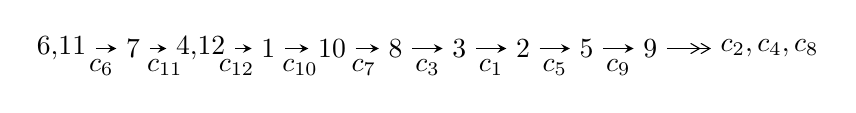
\begin{tikzpicture}[x=23pt, y=7pt]
	% node
	\node (A0) at (-1/8, 0) {6,11};
	\node (A1) at (1, 0) {7};
	\node (A2) at (33/16, 0) {4,12};
	\node (A3) at (25/8, 0) {1};
	\node (A4) at (33/8, 0) {10};
	\node (A5) at (41/8, 0) {8};
	\node (A6) at (49/8, 0) {3};
	\node (A7) at (57/8, 0) {2};
	\node (A8) at (65/8, 0) {5};
	\node (A9) at (73/8, 0) {9};
	\node (C1) at (1/2, -1) {$c_{6}$};
	\node (C2) at (3/2, -1) {$c_{11}$};
	\node (C3) at (21/8, -1) {$c_{12}$};
	\node (C4) at (29/8, -1) {$c_{10}$};
	\node (C5) at (37/8, -1) {$c_{7}$};
	\node (C6) at (45/8, -1) {$c_{3}$};
	\node (C7) at (53/8, -1) {$c_{1}$};
	\node (C8) at (61/8, -1) {$c_{5}$};
	\node (C9) at (69/8, -1) {$c_{9}$};
	\node (A10) at (11, 0) {$c_{2},c_{4},c_{8}$};

	% edge
	\draw[->,>=stealth]	
	(A0) edge (A1) (A1) edge (A2) (A2) edge (A3) (A3) edge (A4) (A4) edge (A5) (A5) edge (A6) (A6) edge (A7) (A7) edge (A8) (A8) edge (A9) ;
	\draw[->>,>={angle 60}]	
	(A9) edge (A10);
\end{tikzpicture} \\ 

\end{tabular} \\

\footnotetext{
The image of knot diagram is generated by the software ``\textbf{Draw programme}" developed by Andrew Bartholomew(\url{http://www.layer8.co.uk/maths/draw/index.htm\#Running-draw}), where we modified some parts for our purpose(\url{https://github.com/CATsTAILs/LinksPainter}).
}\phantom \\ \newline 
\centering \textbf{Ideals for irreducible components\footnotemark of $X_{\text{par}}$} 
 
\begin{align*}
I^u_{1}&=\langle 
1.49803\times10^{58} u^{89}+5.92542\times10^{58} u^{88}+\cdots+1.72660\times10^{59} b+1.98078\times10^{59},\\
\phantom{I^u_{1}}&\phantom{= \langle  }1.02947\times10^{59} u^{89}+2.41879\times10^{58} u^{88}+\cdots+1.72660\times10^{59} a+1.67665\times10^{59},\;u^{90}+u^{89}+\cdots+5 u+1\rangle \\
\\
\end{align*}
\raggedright * 1 irreducible components of $\dim_{\mathbb{C}}=0$, with total 90 representations.\\
\footnotetext{All coefficients of polynomials are rational numbers. But the coefficients are sometimes approximated in decimal forms when there is not enough margin.}
\newpage
\renewcommand{\arraystretch}{1}
\centering \section*{I. $I^u_{1}= \langle 1.50\times10^{58} u^{89}+5.93\times10^{58} u^{88}+\cdots+1.73\times10^{59} b+1.98\times10^{59},\;1.03\times10^{59} u^{89}+2.42\times10^{58} u^{88}+\cdots+1.73\times10^{59} a+1.68\times10^{59},\;u^{90}+u^{89}+\cdots+5 u+1 \rangle$}
\flushleft \textbf{(i) Arc colorings}\\
\begin{tabular}{m{7pt} m{180pt} m{7pt} m{180pt} }
\flushright $a_{6}=$&$\begin{pmatrix}1\\0\end{pmatrix}$ \\
\flushright $a_{11}=$&$\begin{pmatrix}0\\u\end{pmatrix}$ \\
\flushright $a_{7}=$&$\begin{pmatrix}1\\u^2\end{pmatrix}$ \\
\flushright $a_{4}=$&$\begin{pmatrix}-0.596241 u^{89}-0.140090 u^{88}+\cdots-10.1457 u-0.971072\\-0.0867618 u^{89}-0.343185 u^{88}+\cdots-1.42481 u-1.14721\end{pmatrix}$ \\
\flushright $a_{12}=$&$\begin{pmatrix}- u\\u\end{pmatrix}$ \\
\flushright $a_{1}=$&$\begin{pmatrix}0.506491 u^{89}-0.464959 u^{88}+\cdots-2.21593 u+0.951695\\0.858763 u^{89}+0.971450 u^{88}+\cdots+4.50932 u+1.36525\end{pmatrix}$ \\
\flushright $a_{10}=$&$\begin{pmatrix}u\\u^3+u\end{pmatrix}$ \\
\flushright $a_{8}=$&$\begin{pmatrix}u^2+1\\u^4+2 u^2\end{pmatrix}$ \\
\flushright $a_{3}=$&$\begin{pmatrix}-0.922415 u^{89}+0.486437 u^{88}+\cdots-9.28974 u-1.51851\\-0.101016 u^{89}-0.289665 u^{88}+\cdots-6.01833 u-2.17824\end{pmatrix}$ \\
\flushright $a_{2}=$&$\begin{pmatrix}0.598272 u^{89}-0.135672 u^{88}+\cdots-2.38042 u-1.48653\\0.110717 u^{89}+0.268130 u^{88}+\cdots+6.26801 u+1.12390\end{pmatrix}$ \\
\flushright $a_{5}=$&$\begin{pmatrix}-0.653759 u^{89}+0.807509 u^{88}+\cdots-4.03678 u+0.331898\\-0.100166 u^{89}-0.244164 u^{88}+\cdots-5.85636 u-1.97404\end{pmatrix}$ \\
\flushright $a_{9}=$&$\begin{pmatrix}- u^5-2 u^3+u\\u^5+3 u^3+u\end{pmatrix}$\\&\end{tabular}
\flushleft \textbf{(ii) Obstruction class $= -1$}\\~\\
\flushleft \textbf{(iii) Cusp Shapes $= -2.95959 u^{89}-1.57308 u^{88}+\cdots+33.0318 u+12.1521$}\\~\\
\newpage\renewcommand{\arraystretch}{1}
\flushleft \textbf{(iv) u-Polynomials at the component}\newline \\
\begin{tabular}{m{50pt}|m{274pt}}
Crossings & \hspace{64pt}u-Polynomials at each crossing \\
\hline $$\begin{aligned}c_{1}\end{aligned}$$&$\begin{aligned}
&u^{90}+37 u^{89}+\cdots+9 u+1
\end{aligned}$\\
\hline $$\begin{aligned}c_{2},c_{5}\end{aligned}$$&$\begin{aligned}
&u^{90}+u^{89}+\cdots+9 u+1
\end{aligned}$\\
\hline $$\begin{aligned}c_{3}\end{aligned}$$&$\begin{aligned}
&u^{90}- u^{89}+\cdots-21 u+1
\end{aligned}$\\
\hline $$\begin{aligned}c_{4}\end{aligned}$$&$\begin{aligned}
&u^{90}+u^{89}+\cdots+53 u+7
\end{aligned}$\\
\hline $$\begin{aligned}c_{6},c_{7},c_{10}\\c_{11}\end{aligned}$$&$\begin{aligned}
&u^{90}- u^{89}+\cdots-5 u+1
\end{aligned}$\\
\hline $$\begin{aligned}c_{8}\end{aligned}$$&$\begin{aligned}
&u^{90}+5 u^{89}+\cdots+u+1
\end{aligned}$\\
\hline $$\begin{aligned}c_{9}\end{aligned}$$&$\begin{aligned}
&u^{90}+21 u^{89}+\cdots+30261 u+4067
\end{aligned}$\\
\hline $$\begin{aligned}c_{12}\end{aligned}$$&$\begin{aligned}
&u^{90}+9 u^{89}+\cdots+u+1
\end{aligned}$\\
\hline
\end{tabular}\\~\\
\newpage\renewcommand{\arraystretch}{1}
\flushleft \textbf{(v) Riley Polynomials at the component}\newline \\
\begin{tabular}{m{50pt}|m{274pt}}
Crossings & \hspace{64pt}Riley Polynomials at each crossing \\
\hline $$\begin{aligned}c_{1}\end{aligned}$$&$\begin{aligned}
&y^{90}+33 y^{89}+\cdots-403 y+1
\end{aligned}$\\
\hline $$\begin{aligned}c_{2},c_{5}\end{aligned}$$&$\begin{aligned}
&y^{90}+37 y^{89}+\cdots+9 y+1
\end{aligned}$\\
\hline $$\begin{aligned}c_{3}\end{aligned}$$&$\begin{aligned}
&y^{90}+101 y^{89}+\cdots+89 y+1
\end{aligned}$\\
\hline $$\begin{aligned}c_{4}\end{aligned}$$&$\begin{aligned}
&y^{90}+93 y^{89}+\cdots+1237 y+49
\end{aligned}$\\
\hline $$\begin{aligned}c_{6},c_{7},c_{10}\\c_{11}\end{aligned}$$&$\begin{aligned}
&y^{90}+101 y^{89}+\cdots+5 y+1
\end{aligned}$\\
\hline $$\begin{aligned}c_{8}\end{aligned}$$&$\begin{aligned}
&y^{90}+9 y^{89}+\cdots+5 y+1
\end{aligned}$\\
\hline $$\begin{aligned}c_{9}\end{aligned}$$&$\begin{aligned}
&y^{90}+13 y^{89}+\cdots+583522625 y+16540489
\end{aligned}$\\
\hline $$\begin{aligned}c_{12}\end{aligned}$$&$\begin{aligned}
&y^{90}+5 y^{89}+\cdots+9 y+1
\end{aligned}$\\
\hline
\end{tabular}\\~\\
\newpage\flushleft \textbf{(vi) Complex Volumes and Cusp Shapes}
$$\begin{array}{c|c|c}  
\text{Solutions to }I^u_{1}& \I (\text{vol} + \sqrt{-1}CS) & \text{Cusp shape}\\
 \hline 
\begin{aligned}
u &= -0.153386 + 0.949459 I \\
a &= \phantom{-}0.718759 + 0.923313 I \\
b &= \phantom{-}0.174097 - 0.184217 I\end{aligned}
 & \phantom{-}4.37025 - 2.09737 I & \phantom{-0.000000 } 0 \\ \hline\begin{aligned}
u &= -0.153386 - 0.949459 I \\
a &= \phantom{-}0.718759 - 0.923313 I \\
b &= \phantom{-}0.174097 + 0.184217 I\end{aligned}
 & \phantom{-}4.37025 + 2.09737 I & \phantom{-0.000000 } 0 \\ \hline\begin{aligned}
u &= \phantom{-}0.592585 + 0.748622 I \\
a &= \phantom{-}0.525999 - 0.073835 I \\
b &= -0.247712 + 0.718060 I\end{aligned}
 & -1.04239 - 5.87786 I & \phantom{-0.000000 } 0 \\ \hline\begin{aligned}
u &= \phantom{-}0.592585 - 0.748622 I \\
a &= \phantom{-}0.525999 + 0.073835 I \\
b &= -0.247712 - 0.718060 I\end{aligned}
 & -1.04239 + 5.87786 I & \phantom{-0.000000 } 0 \\ \hline\begin{aligned}
u &= -0.574662 + 0.686016 I \\
a &= \phantom{-}1.314030 + 0.037343 I \\
b &= -1.09112 - 1.69898 I\end{aligned}
 & -0.2793 + 14.4752 I & \phantom{-0.000000 } 0 \\ \hline\begin{aligned}
u &= -0.574662 - 0.686016 I \\
a &= \phantom{-}1.314030 - 0.037343 I \\
b &= -1.09112 + 1.69898 I\end{aligned}
 & -0.2793 - 14.4752 I & \phantom{-0.000000 } 0 \\ \hline\begin{aligned}
u &= -0.150469 + 1.111890 I \\
a &= -0.878713 - 0.860540 I \\
b &= \phantom{-}0.042720 + 0.283468 I\end{aligned}
 & \phantom{-}2.83318 - 7.25186 I & \phantom{-0.000000 } 0 \\ \hline\begin{aligned}
u &= -0.150469 - 1.111890 I \\
a &= -0.878713 + 0.860540 I \\
b &= \phantom{-}0.042720 - 0.283468 I\end{aligned}
 & \phantom{-}2.83318 + 7.25186 I & \phantom{-0.000000 } 0 \\ \hline\begin{aligned}
u &= \phantom{-}0.417484 + 0.766577 I \\
a &= -0.398067 - 0.023582 I \\
b &= \phantom{-}0.098415 - 0.679860 I\end{aligned}
 & \phantom{-}0.01934 - 1.98738 I & \phantom{-0.000000 } 0 \\ \hline\begin{aligned}
u &= \phantom{-}0.417484 - 0.766577 I \\
a &= -0.398067 + 0.023582 I \\
b &= \phantom{-}0.098415 + 0.679860 I\end{aligned}
 & \phantom{-}0.01934 + 1.98738 I & \phantom{-0.000000 } 0\\
 \hline 
 \end{array}$$\newpage$$\begin{array}{c|c|c}  
\text{Solutions to }I^u_{1}& \I (\text{vol} + \sqrt{-1}CS) & \text{Cusp shape}\\
 \hline 
\begin{aligned}
u &= -0.540546 + 0.681468 I \\
a &= -1.409290 + 0.010881 I \\
b &= \phantom{-}1.10186 + 1.70068 I\end{aligned}
 & \phantom{-}1.74657 + 8.70254 I & \phantom{-0.000000 } 0 \\ \hline\begin{aligned}
u &= -0.540546 - 0.681468 I \\
a &= -1.409290 - 0.010881 I \\
b &= \phantom{-}1.10186 - 1.70068 I\end{aligned}
 & \phantom{-}1.74657 - 8.70254 I & \phantom{-0.000000 } 0 \\ \hline\begin{aligned}
u &= \phantom{-}0.656158 + 0.547764 I \\
a &= \phantom{-}0.572560 - 0.062751 I \\
b &= -0.313753 + 0.727781 I\end{aligned}
 & -2.06605 - 0.65625 I & \phantom{-0.000000 } 0 \\ \hline\begin{aligned}
u &= \phantom{-}0.656158 - 0.547764 I \\
a &= \phantom{-}0.572560 + 0.062751 I \\
b &= -0.313753 - 0.727781 I\end{aligned}
 & -2.06605 + 0.65625 I & \phantom{-0.000000 } 0 \\ \hline\begin{aligned}
u &= \phantom{-}0.716623 + 0.371946 I \\
a &= -0.498659 - 0.100748 I \\
b &= \phantom{-}0.272381 - 0.633490 I\end{aligned}
 & -2.58726 - 3.92694 I & -12.8588 + 9.2593 I \\ \hline\begin{aligned}
u &= \phantom{-}0.716623 - 0.371946 I \\
a &= -0.498659 + 0.100748 I \\
b &= \phantom{-}0.272381 + 0.633490 I\end{aligned}
 & -2.58726 + 3.92694 I & -12.8588 - 9.2593 I \\ \hline\begin{aligned}
u &= -0.531750 + 0.597942 I \\
a &= \phantom{-}1.328430 - 0.323224 I \\
b &= -1.13869 - 1.67077 I\end{aligned}
 & -4.62635 + 6.13378 I & \phantom{-0.000000 } 0. - 8.46328 I \\ \hline\begin{aligned}
u &= -0.531750 - 0.597942 I \\
a &= \phantom{-}1.328430 + 0.323224 I \\
b &= -1.13869 + 1.67077 I\end{aligned}
 & -4.62635 - 6.13378 I & \phantom{-0.000000 -}0. + 8.46328 I \\ \hline\begin{aligned}
u &= -0.443199 + 0.608183 I \\
a &= -1.21211 - 1.52602 I \\
b &= -0.912945 + 0.867545 I\end{aligned}
 & \phantom{-}0.35574 + 6.37386 I & \phantom{-}1.05559 - 12.60773 I \\ \hline\begin{aligned}
u &= -0.443199 - 0.608183 I \\
a &= -1.21211 + 1.52602 I \\
b &= -0.912945 - 0.867545 I\end{aligned}
 & \phantom{-}0.35574 - 6.37386 I & \phantom{-}1.05559 + 12.60773 I\\
 \hline 
 \end{array}$$\newpage$$\begin{array}{c|c|c}  
\text{Solutions to }I^u_{1}& \I (\text{vol} + \sqrt{-1}CS) & \text{Cusp shape}\\
 \hline 
\begin{aligned}
u &= \phantom{-}0.387123 + 0.636739 I \\
a &= -0.193637 + 0.190795 I \\
b &= -0.006821 - 0.901193 I\end{aligned}
 & -0.01272 - 2.08828 I & -2.58132 + 5.68138 I \\ \hline\begin{aligned}
u &= \phantom{-}0.387123 - 0.636739 I \\
a &= -0.193637 - 0.190795 I \\
b &= -0.006821 + 0.901193 I\end{aligned}
 & -0.01272 + 2.08828 I & -2.58132 - 5.68138 I \\ \hline\begin{aligned}
u &= -0.375933 + 0.626578 I \\
a &= -2.06776 + 0.11377 I \\
b &= \phantom{-}1.01204 + 1.77494 I\end{aligned}
 & \phantom{-}2.64454 + 3.98095 I & \phantom{-}7.57746 - 9.49711 I \\ \hline\begin{aligned}
u &= -0.375933 - 0.626578 I \\
a &= -2.06776 - 0.11377 I \\
b &= \phantom{-}1.01204 - 1.77494 I\end{aligned}
 & \phantom{-}2.64454 - 3.98095 I & \phantom{-}7.57746 + 9.49711 I \\ \hline\begin{aligned}
u &= -0.669369 + 0.250763 I \\
a &= -1.249650 - 0.365953 I \\
b &= -0.458430 + 1.299980 I\end{aligned}
 & -1.56816 - 10.28520 I & -3.97736 + 6.02657 I \\ \hline\begin{aligned}
u &= -0.669369 - 0.250763 I \\
a &= -1.249650 + 0.365953 I \\
b &= -0.458430 - 1.299980 I\end{aligned}
 & -1.56816 + 10.28520 I & -3.97736 - 6.02657 I \\ \hline\begin{aligned}
u &= \phantom{-}0.703492 + 0.126133 I \\
a &= -0.222901 - 0.350127 I \\
b &= \phantom{-}0.112898 - 0.515008 I\end{aligned}
 & -2.86278 + 1.53210 I & -14.6011 - 1.5393 I \\ \hline\begin{aligned}
u &= \phantom{-}0.703492 - 0.126133 I \\
a &= -0.222901 + 0.350127 I \\
b &= \phantom{-}0.112898 + 0.515008 I\end{aligned}
 & -2.86278 - 1.53210 I & -14.6011 + 1.5393 I \\ \hline\begin{aligned}
u &= -0.317537 + 0.631586 I \\
a &= \phantom{-}0.69364 + 1.58671 I \\
b &= \phantom{-}0.928055 - 0.324587 I\end{aligned}
 & \phantom{-}2.99128 + 0.66231 I & \phantom{-}9.52889 - 2.63944 I \\ \hline\begin{aligned}
u &= -0.317537 - 0.631586 I \\
a &= \phantom{-}0.69364 - 1.58671 I \\
b &= \phantom{-}0.928055 + 0.324587 I\end{aligned}
 & \phantom{-}2.99128 - 0.66231 I & \phantom{-}9.52889 + 2.63944 I\\
 \hline 
 \end{array}$$\newpage$$\begin{array}{c|c|c}  
\text{Solutions to }I^u_{1}& \I (\text{vol} + \sqrt{-1}CS) & \text{Cusp shape}\\
 \hline 
\begin{aligned}
u &= \phantom{-}0.165064 + 1.288320 I \\
a &= -1.113030 - 0.351119 I \\
b &= \phantom{-}0.563002 - 0.110438 I\end{aligned}
 & \phantom{-}2.63709 - 7.22205 I & \phantom{-0.000000 } 0 \\ \hline\begin{aligned}
u &= \phantom{-}0.165064 - 1.288320 I \\
a &= -1.113030 + 0.351119 I \\
b &= \phantom{-}0.563002 + 0.110438 I\end{aligned}
 & \phantom{-}2.63709 + 7.22205 I & \phantom{-0.000000 } 0 \\ \hline\begin{aligned}
u &= \phantom{-}0.418563 + 0.546343 I \\
a &= -2.50765 - 0.56009 I \\
b &= \phantom{-}1.94029 + 0.73720 I\end{aligned}
 & -0.24570 - 3.76742 I & \phantom{-}2.5969 - 21.3357 I \\ \hline\begin{aligned}
u &= \phantom{-}0.418563 - 0.546343 I \\
a &= -2.50765 + 0.56009 I \\
b &= \phantom{-}1.94029 - 0.73720 I\end{aligned}
 & -0.24570 + 3.76742 I & \phantom{-}2.5969 + 21.3357 I \\ \hline\begin{aligned}
u &= -0.569753 + 0.342177 I \\
a &= -1.57369 - 0.51879 I \\
b &= -0.457247 + 1.318270 I\end{aligned}
 & -5.37588 - 2.34777 I & -8.46003 + 1.41530 I \\ \hline\begin{aligned}
u &= -0.569753 - 0.342177 I \\
a &= -1.57369 + 0.51879 I \\
b &= -0.457247 - 1.318270 I\end{aligned}
 & -5.37588 + 2.34777 I & -8.46003 - 1.41530 I \\ \hline\begin{aligned}
u &= -0.622072 + 0.229860 I \\
a &= \phantom{-}1.333090 + 0.265168 I \\
b &= \phantom{-}0.458059 - 1.289570 I\end{aligned}
 & \phantom{-}0.42234 - 4.75738 I & -1.60038 + 2.22004 I \\ \hline\begin{aligned}
u &= -0.622072 - 0.229860 I \\
a &= \phantom{-}1.333090 - 0.265168 I \\
b &= \phantom{-}0.458059 + 1.289570 I\end{aligned}
 & \phantom{-}0.42234 + 4.75738 I & -1.60038 - 2.22004 I \\ \hline\begin{aligned}
u &= \phantom{-}0.351415 + 0.558810 I \\
a &= \phantom{-}2.39621 + 0.42195 I \\
b &= -1.69911 - 0.46842 I\end{aligned}
 & \phantom{-}0.133011 + 0.337575 I & -11.1760 - 9.1703 I \\ \hline\begin{aligned}
u &= \phantom{-}0.351415 - 0.558810 I \\
a &= \phantom{-}2.39621 - 0.42195 I \\
b &= -1.69911 + 0.46842 I\end{aligned}
 & \phantom{-}0.133011 - 0.337575 I & -11.1760 + 9.1703 I\\
 \hline 
 \end{array}$$\newpage$$\begin{array}{c|c|c}  
\text{Solutions to }I^u_{1}& \I (\text{vol} + \sqrt{-1}CS) & \text{Cusp shape}\\
 \hline 
\begin{aligned}
u &= -0.220551 + 0.576106 I \\
a &= \phantom{-}2.35810 + 0.27719 I \\
b &= -0.74063 - 1.49851 I\end{aligned}
 & \phantom{-}1.73042 - 2.10860 I & \phantom{-}6.00206 + 2.72036 I \\ \hline\begin{aligned}
u &= -0.220551 - 0.576106 I \\
a &= \phantom{-}2.35810 - 0.27719 I \\
b &= -0.74063 + 1.49851 I\end{aligned}
 & \phantom{-}1.73042 + 2.10860 I & \phantom{-}6.00206 - 2.72036 I \\ \hline\begin{aligned}
u &= \phantom{-}0.407501 + 0.439459 I \\
a &= -1.91928 - 0.47694 I \\
b &= \phantom{-}1.40687 + 0.99133 I\end{aligned}
 & -0.571516 + 0.804092 I & \phantom{-}14.6443 + 7.0088 I \\ \hline\begin{aligned}
u &= \phantom{-}0.407501 - 0.439459 I \\
a &= -1.91928 + 0.47694 I \\
b &= \phantom{-}1.40687 - 0.99133 I\end{aligned}
 & -0.571516 - 0.804092 I & \phantom{-}14.6443 - 7.0088 I \\ \hline\begin{aligned}
u &= \phantom{-}0.05663 + 1.42405 I \\
a &= \phantom{-}1.58377 + 0.57387 I \\
b &= -0.963257 - 0.289901 I\end{aligned}
 & \phantom{-}4.57161 - 2.79628 I & \phantom{-0.000000 } 0 \\ \hline\begin{aligned}
u &= \phantom{-}0.05663 - 1.42405 I \\
a &= \phantom{-}1.58377 - 0.57387 I \\
b &= -0.963257 + 0.289901 I\end{aligned}
 & \phantom{-}4.57161 + 2.79628 I & \phantom{-0.000000 } 0 \\ \hline\begin{aligned}
u &= \phantom{-}0.471994 + 0.317933 I \\
a &= \phantom{-}0.952599 + 0.435782 I \\
b &= -0.484844 + 0.384289 I\end{aligned}
 & -0.989919 - 0.990182 I & -5.04840 + 4.14744 I \\ \hline\begin{aligned}
u &= \phantom{-}0.471994 - 0.317933 I \\
a &= \phantom{-}0.952599 - 0.435782 I \\
b &= -0.484844 - 0.384289 I\end{aligned}
 & -0.989919 + 0.990182 I & -5.04840 - 4.14744 I \\ \hline\begin{aligned}
u &= -0.09077 + 1.42884 I \\
a &= -1.29677 - 1.10983 I \\
b &= \phantom{-}0.450417 + 0.767926 I\end{aligned}
 & \phantom{-}0.201142 - 0.116256 I & \phantom{-0.000000 } 0 \\ \hline\begin{aligned}
u &= -0.09077 - 1.42884 I \\
a &= -1.29677 + 1.10983 I \\
b &= \phantom{-}0.450417 - 0.767926 I\end{aligned}
 & \phantom{-}0.201142 + 0.116256 I & \phantom{-0.000000 } 0\\
 \hline 
 \end{array}$$\newpage$$\begin{array}{c|c|c}  
\text{Solutions to }I^u_{1}& \I (\text{vol} + \sqrt{-1}CS) & \text{Cusp shape}\\
 \hline 
\begin{aligned}
u &= -0.405371 + 0.280603 I \\
a &= -0.199952 - 1.378270 I \\
b &= -0.959262 - 0.968605 I\end{aligned}
 & -0.56516 - 3.28407 I & -3.30805 + 5.23829 I \\ \hline\begin{aligned}
u &= -0.405371 - 0.280603 I \\
a &= -0.199952 + 1.378270 I \\
b &= -0.959262 + 0.968605 I\end{aligned}
 & -0.56516 + 3.28407 I & -3.30805 - 5.23829 I \\ \hline\begin{aligned}
u &= \phantom{-}0.16937 + 1.52158 I \\
a &= \phantom{-}1.51766 - 0.30903 I \\
b &= -1.130990 + 0.625814 I\end{aligned}
 & \phantom{-}4.65622 - 3.58702 I & \phantom{-0.000000 } 0 \\ \hline\begin{aligned}
u &= \phantom{-}0.16937 - 1.52158 I \\
a &= \phantom{-}1.51766 + 0.30903 I \\
b &= -1.130990 - 0.625814 I\end{aligned}
 & \phantom{-}4.65622 + 3.58702 I & \phantom{-0.000000 } 0 \\ \hline\begin{aligned}
u &= \phantom{-}0.09271 + 1.53236 I \\
a &= -1.27280 - 2.03682 I \\
b &= \phantom{-}1.17772 + 2.44286 I\end{aligned}
 & \phantom{-}6.09255 - 0.84757 I & \phantom{-0.000000 } 0 \\ \hline\begin{aligned}
u &= \phantom{-}0.09271 - 1.53236 I \\
a &= -1.27280 + 2.03682 I \\
b &= \phantom{-}1.17772 - 2.44286 I\end{aligned}
 & \phantom{-}6.09255 + 0.84757 I & \phantom{-0.000000 } 0 \\ \hline\begin{aligned}
u &= -0.05357 + 1.53456 I \\
a &= \phantom{-}1.45113 + 0.11741 I \\
b &= -1.46172 - 1.07706 I\end{aligned}
 & \phantom{-}5.68381 - 2.27432 I & \phantom{-0.000000 } 0 \\ \hline\begin{aligned}
u &= -0.05357 - 1.53456 I \\
a &= \phantom{-}1.45113 - 0.11741 I \\
b &= -1.46172 + 1.07706 I\end{aligned}
 & \phantom{-}5.68381 + 2.27432 I & \phantom{-0.000000 } 0 \\ \hline\begin{aligned}
u &= \phantom{-}0.11432 + 1.56167 I \\
a &= -2.93352 - 1.95251 I \\
b &= \phantom{-}2.65903 + 2.16225 I\end{aligned}
 & \phantom{-}6.90903 - 5.66157 I & \phantom{-0.000000 } 0 \\ \hline\begin{aligned}
u &= \phantom{-}0.11432 - 1.56167 I \\
a &= -2.93352 + 1.95251 I \\
b &= \phantom{-}2.65903 - 2.16225 I\end{aligned}
 & \phantom{-}6.90903 + 5.66157 I & \phantom{-0.000000 } 0\\
 \hline 
 \end{array}$$\newpage$$\begin{array}{c|c|c}  
\text{Solutions to }I^u_{1}& \I (\text{vol} + \sqrt{-1}CS) & \text{Cusp shape}\\
 \hline 
\begin{aligned}
u &= \phantom{-}0.09617 + 1.56590 I \\
a &= \phantom{-}3.12411 + 1.27896 I \\
b &= -2.77213 - 1.39716 I\end{aligned}
 & \phantom{-}7.37300 - 1.26295 I & \phantom{-0.000000 } 0 \\ \hline\begin{aligned}
u &= \phantom{-}0.09617 - 1.56590 I \\
a &= \phantom{-}3.12411 - 1.27896 I \\
b &= -2.77213 + 1.39716 I\end{aligned}
 & \phantom{-}7.37300 + 1.26295 I & \phantom{-0.000000 } 0 \\ \hline\begin{aligned}
u &= -0.15237 + 1.56573 I \\
a &= \phantom{-}2.50255 + 1.03565 I \\
b &= -1.82102 - 1.91169 I\end{aligned}
 & \phantom{-}2.62908 + 8.61485 I & \phantom{-0.000000 } 0 \\ \hline\begin{aligned}
u &= -0.15237 - 1.56573 I \\
a &= \phantom{-}2.50255 - 1.03565 I \\
b &= -1.82102 + 1.91169 I\end{aligned}
 & \phantom{-}2.62908 - 8.61485 I & \phantom{-0.000000 } 0 \\ \hline\begin{aligned}
u &= -0.07670 + 1.57131 I \\
a &= \phantom{-}2.36617 + 1.61202 I \\
b &= -1.31873 - 1.95306 I\end{aligned}
 & \phantom{-}9.07886 - 0.93094 I & \phantom{-0.000000 } 0 \\ \hline\begin{aligned}
u &= -0.07670 - 1.57131 I \\
a &= \phantom{-}2.36617 - 1.61202 I \\
b &= -1.31873 + 1.95306 I\end{aligned}
 & \phantom{-}9.07886 + 0.93094 I & \phantom{-0.000000 } 0 \\ \hline\begin{aligned}
u &= -0.12500 + 1.57476 I \\
a &= \phantom{-}0.06493 - 1.49401 I \\
b &= -0.906132 + 0.621652 I\end{aligned}
 & \phantom{-}7.74476 + 8.43784 I & \phantom{-0.000000 } 0 \\ \hline\begin{aligned}
u &= -0.12500 - 1.57476 I \\
a &= \phantom{-}0.06493 + 1.49401 I \\
b &= -0.906132 - 0.621652 I\end{aligned}
 & \phantom{-}7.74476 - 8.43784 I & \phantom{-0.000000 } 0 \\ \hline\begin{aligned}
u &= \phantom{-}0.10144 + 1.57704 I \\
a &= -0.66918 + 1.52360 I \\
b &= \phantom{-}0.49284 - 1.89219 I\end{aligned}
 & \phantom{-}7.47987 - 3.80306 I & \phantom{-0.000000 } 0 \\ \hline\begin{aligned}
u &= \phantom{-}0.10144 - 1.57704 I \\
a &= -0.66918 - 1.52360 I \\
b &= \phantom{-}0.49284 + 1.89219 I\end{aligned}
 & \phantom{-}7.47987 + 3.80306 I & \phantom{-0.000000 } 0\\
 \hline 
 \end{array}$$\newpage$$\begin{array}{c|c|c}  
\text{Solutions to }I^u_{1}& \I (\text{vol} + \sqrt{-1}CS) & \text{Cusp shape}\\
 \hline 
\begin{aligned}
u &= -0.09384 + 1.58164 I \\
a &= -0.702815 + 1.007970 I \\
b &= \phantom{-}1.244420 + 0.005868 I\end{aligned}
 & \phantom{-}10.52950 + 2.19494 I & \phantom{-0.000000 } 0 \\ \hline\begin{aligned}
u &= -0.09384 - 1.58164 I \\
a &= -0.702815 - 1.007970 I \\
b &= \phantom{-}1.244420 - 0.005868 I\end{aligned}
 & \phantom{-}10.52950 - 2.19494 I & \phantom{-0.000000 } 0 \\ \hline\begin{aligned}
u &= -0.10790 + 1.58110 I \\
a &= -2.64329 - 1.41564 I \\
b &= \phantom{-}1.66442 + 2.10196 I\end{aligned}
 & \phantom{-}10.15180 + 5.76027 I & \phantom{-0.000000 } 0 \\ \hline\begin{aligned}
u &= -0.10790 - 1.58110 I \\
a &= -2.64329 + 1.41564 I \\
b &= \phantom{-}1.66442 - 2.10196 I\end{aligned}
 & \phantom{-}10.15180 - 5.76027 I & \phantom{-0.000000 } 0 \\ \hline\begin{aligned}
u &= -0.16145 + 1.59638 I \\
a &= -2.42197 - 1.17248 I \\
b &= \phantom{-}1.75629 + 1.92985 I\end{aligned}
 & \phantom{-}9.4286 + 11.3153 I & \phantom{-0.000000 } 0 \\ \hline\begin{aligned}
u &= -0.16145 - 1.59638 I \\
a &= -2.42197 + 1.17248 I \\
b &= \phantom{-}1.75629 - 1.92985 I\end{aligned}
 & \phantom{-}9.4286 - 11.3153 I & \phantom{-0.000000 } 0 \\ \hline\begin{aligned}
u &= -0.17437 + 1.59798 I \\
a &= \phantom{-}2.37867 + 1.16311 I \\
b &= -1.74876 - 1.91913 I\end{aligned}
 & \phantom{-}7.4050 + 17.2703 I & \phantom{-0.000000 } 0 \\ \hline\begin{aligned}
u &= -0.17437 - 1.59798 I \\
a &= \phantom{-}2.37867 - 1.16311 I \\
b &= -1.74876 + 1.91913 I\end{aligned}
 & \phantom{-}7.4050 - 17.2703 I & \phantom{-0.000000 } 0 \\ \hline\begin{aligned}
u &= \phantom{-}0.14486 + 1.61314 I \\
a &= -0.922533 + 0.684068 I \\
b &= \phantom{-}0.625007 - 1.078630 I\end{aligned}
 & \phantom{-}8.05248 - 4.24619 I & \phantom{-0.000000 } 0 \\ \hline\begin{aligned}
u &= \phantom{-}0.14486 - 1.61314 I \\
a &= -0.922533 - 0.684068 I \\
b &= \phantom{-}0.625007 + 1.078630 I\end{aligned}
 & \phantom{-}8.05248 + 4.24619 I & \phantom{-0.000000 } 0\\
 \hline 
 \end{array}$$\newpage$$\begin{array}{c|c|c}  
\text{Solutions to }I^u_{1}& \I (\text{vol} + \sqrt{-1}CS) & \text{Cusp shape}\\
 \hline 
\begin{aligned}
u &= \phantom{-}0.18353 + 1.61376 I \\
a &= \phantom{-}1.027430 - 0.490906 I \\
b &= -0.695784 + 0.881112 I\end{aligned}
 & \phantom{-}6.89750 - 8.82487 I & \phantom{-0.000000 } 0 \\ \hline\begin{aligned}
u &= \phantom{-}0.18353 - 1.61376 I \\
a &= \phantom{-}1.027430 + 0.490906 I \\
b &= -0.695784 - 0.881112 I\end{aligned}
 & \phantom{-}6.89750 + 8.82487 I & \phantom{-0.000000 } 0 \\ \hline\begin{aligned}
u &= \phantom{-}0.227195 + 0.284908 I \\
a &= \phantom{-}1.90995 - 0.81708 I \\
b &= -0.954823 - 0.478011 I\end{aligned}
 & -0.50806 - 2.64460 I & \phantom{-}2.81091 + 6.46234 I \\ \hline\begin{aligned}
u &= \phantom{-}0.227195 - 0.284908 I \\
a &= \phantom{-}1.90995 + 0.81708 I \\
b &= -0.954823 + 0.478011 I\end{aligned}
 & -0.50806 + 2.64460 I & \phantom{-}2.81091 - 6.46234 I \\ \hline\begin{aligned}
u &= -0.02421 + 1.64276 I \\
a &= -0.0903645 + 0.0173208 I \\
b &= \phantom{-}0.439641 + 0.634212 I\end{aligned}
 & \phantom{-}13.23290 - 1.53819 I & \phantom{-0.000000 } 0 \\ \hline\begin{aligned}
u &= -0.02421 - 1.64276 I \\
a &= -0.0903645 - 0.0173208 I \\
b &= \phantom{-}0.439641 - 0.634212 I\end{aligned}
 & \phantom{-}13.23290 + 1.53819 I & \phantom{-0.000000 } 0 \\ \hline\begin{aligned}
u &= -0.339095 + 0.048393 I \\
a &= \phantom{-}1.85470 - 0.96460 I \\
b &= \phantom{-}0.425963 - 0.989713 I\end{aligned}
 & \phantom{-}1.24876 - 1.48001 I & \phantom{-}1.04199 + 3.33888 I \\ \hline\begin{aligned}
u &= -0.339095 - 0.048393 I \\
a &= \phantom{-}1.85470 + 0.96460 I \\
b &= \phantom{-}0.425963 + 0.989713 I\end{aligned}
 & \phantom{-}1.24876 + 1.48001 I & \phantom{-}1.04199 - 3.33888 I \\ \hline\begin{aligned}
u &= -0.00034 + 1.65939 I \\
a &= -0.0768283 + 0.1112280 I \\
b &= -0.262523 - 0.705756 I\end{aligned}
 & \phantom{-}12.22560 - 7.06179 I & \phantom{-0.000000 } 0 \\ \hline\begin{aligned}
u &= -0.00034 - 1.65939 I \\
a &= -0.0768283 - 0.1112280 I \\
b &= -0.262523 + 0.705756 I\end{aligned}
 & \phantom{-}12.22560 + 7.06179 I & \phantom{-0.000000 } 0\\
 \hline 
 \end{array}$$\newpage
\newpage\renewcommand{\arraystretch}{1}
\centering \section*{ II. u-Polynomials}
\begin{tabular}{m{50pt}|m{274pt}}
Crossings & \hspace{64pt}u-Polynomials at each crossing \\
\hline $$\begin{aligned}c_{1}\end{aligned}$$&$\begin{aligned}
&u^{90}+37 u^{89}+\cdots+9 u+1
\end{aligned}$\\
\hline $$\begin{aligned}c_{2},c_{5}\end{aligned}$$&$\begin{aligned}
&u^{90}+u^{89}+\cdots+9 u+1
\end{aligned}$\\
\hline $$\begin{aligned}c_{3}\end{aligned}$$&$\begin{aligned}
&u^{90}- u^{89}+\cdots-21 u+1
\end{aligned}$\\
\hline $$\begin{aligned}c_{4}\end{aligned}$$&$\begin{aligned}
&u^{90}+u^{89}+\cdots+53 u+7
\end{aligned}$\\
\hline $$\begin{aligned}c_{6},c_{7},c_{10}\\c_{11}\end{aligned}$$&$\begin{aligned}
&u^{90}- u^{89}+\cdots-5 u+1
\end{aligned}$\\
\hline $$\begin{aligned}c_{8}\end{aligned}$$&$\begin{aligned}
&u^{90}+5 u^{89}+\cdots+u+1
\end{aligned}$\\
\hline $$\begin{aligned}c_{9}\end{aligned}$$&$\begin{aligned}
&u^{90}+21 u^{89}+\cdots+30261 u+4067
\end{aligned}$\\
\hline $$\begin{aligned}c_{12}\end{aligned}$$&$\begin{aligned}
&u^{90}+9 u^{89}+\cdots+u+1
\end{aligned}$\\
\hline
\end{tabular}\newpage\renewcommand{\arraystretch}{1}
\centering \section*{ III. Riley Polynomials}
\begin{tabular}{m{50pt}|m{274pt}}
Crossings & \hspace{64pt}Riley Polynomials at each crossing \\
\hline $$\begin{aligned}c_{1}\end{aligned}$$&$\begin{aligned}
&y^{90}+33 y^{89}+\cdots-403 y+1
\end{aligned}$\\
\hline $$\begin{aligned}c_{2},c_{5}\end{aligned}$$&$\begin{aligned}
&y^{90}+37 y^{89}+\cdots+9 y+1
\end{aligned}$\\
\hline $$\begin{aligned}c_{3}\end{aligned}$$&$\begin{aligned}
&y^{90}+101 y^{89}+\cdots+89 y+1
\end{aligned}$\\
\hline $$\begin{aligned}c_{4}\end{aligned}$$&$\begin{aligned}
&y^{90}+93 y^{89}+\cdots+1237 y+49
\end{aligned}$\\
\hline $$\begin{aligned}c_{6},c_{7},c_{10}\\c_{11}\end{aligned}$$&$\begin{aligned}
&y^{90}+101 y^{89}+\cdots+5 y+1
\end{aligned}$\\
\hline $$\begin{aligned}c_{8}\end{aligned}$$&$\begin{aligned}
&y^{90}+9 y^{89}+\cdots+5 y+1
\end{aligned}$\\
\hline $$\begin{aligned}c_{9}\end{aligned}$$&$\begin{aligned}
&y^{90}+13 y^{89}+\cdots+583522625 y+16540489
\end{aligned}$\\
\hline $$\begin{aligned}c_{12}\end{aligned}$$&$\begin{aligned}
&y^{90}+5 y^{89}+\cdots+9 y+1
\end{aligned}$\\
\hline
\end{tabular}
\vskip 2pc
\end{document}